\documentclass[12pt]{article}
\usepackage{graphicx}
\usepackage{xcolor}
\usepackage{subcaption}

\usepackage{hyperref}
\definecolor{linkcolour}{rgb}{0,0,1}

\hypersetup{colorlinks=True, 
		urlcolor=linkcolour,
		pdfborderstyle={/S/U/W 2}} 

\usepackage{setspace} 
\singlespacing

\usepackage{geometry}
\geometry{margin=0.5in}

\setlength\parindent{0pt}

\graphicspath{{images/}}

\begin{document}
\title{Bike-Share Case Study}
\date{}
\maketitle

This report provides the step-by-step explanation of the data analysis performed for a bike-sharing case study. The data belongs to a company that has two kinds of users: annual members and casual riders. The aim of the marketing team is to convert casual riders into annual members in the next campaign. Thus, the goal of the study was to identify how annual members and casual riders use the bikes differently in order to provide the marketing team with insights. The data on which the analysis was carried out is from January-December 2023 and was downloaded from \href{https://divvy-tripdata.s3.amazonaws.com/index.html}{\underline{here}}. The library Pandas from Python was used to perform the analysis, and Matplotlib was used to plot the results. The code can be found in the Jupyter Notebook \href{https://github.com/SummerKassem/BikeShareCS/blob/main/PythonCode/bike_share_analysis.ipynb}{\underline{here}}. The structure of the report consists of the following:
\begin{enumerate} 
	\item Importing
	\item Exploration
	\item Cleaning
	\item Preparation
	\item Analysis
	\item Conclusion
\end{enumerate}

\section{Importing}

The original data as downloaded from \href{https://divvy-tripdata.s3.amazonaws.com/index.html}{\underline{here}}, consists of 12 .csv files. So first, each file is read and stored into a DataFrame (DF), and then all 12 DFs are concatenated into a multi-index DF. Using a multi-index DF allows the distinction between the different months to still be maintained, while also facilitating the aggregation of values across the entire year when needed. In Figure (\underline{\ref{fig1}}) we can see the first and last 5 entries of bike rides from the concatenated multi-index DF:

	\begin{figure}[h]
	\centering
	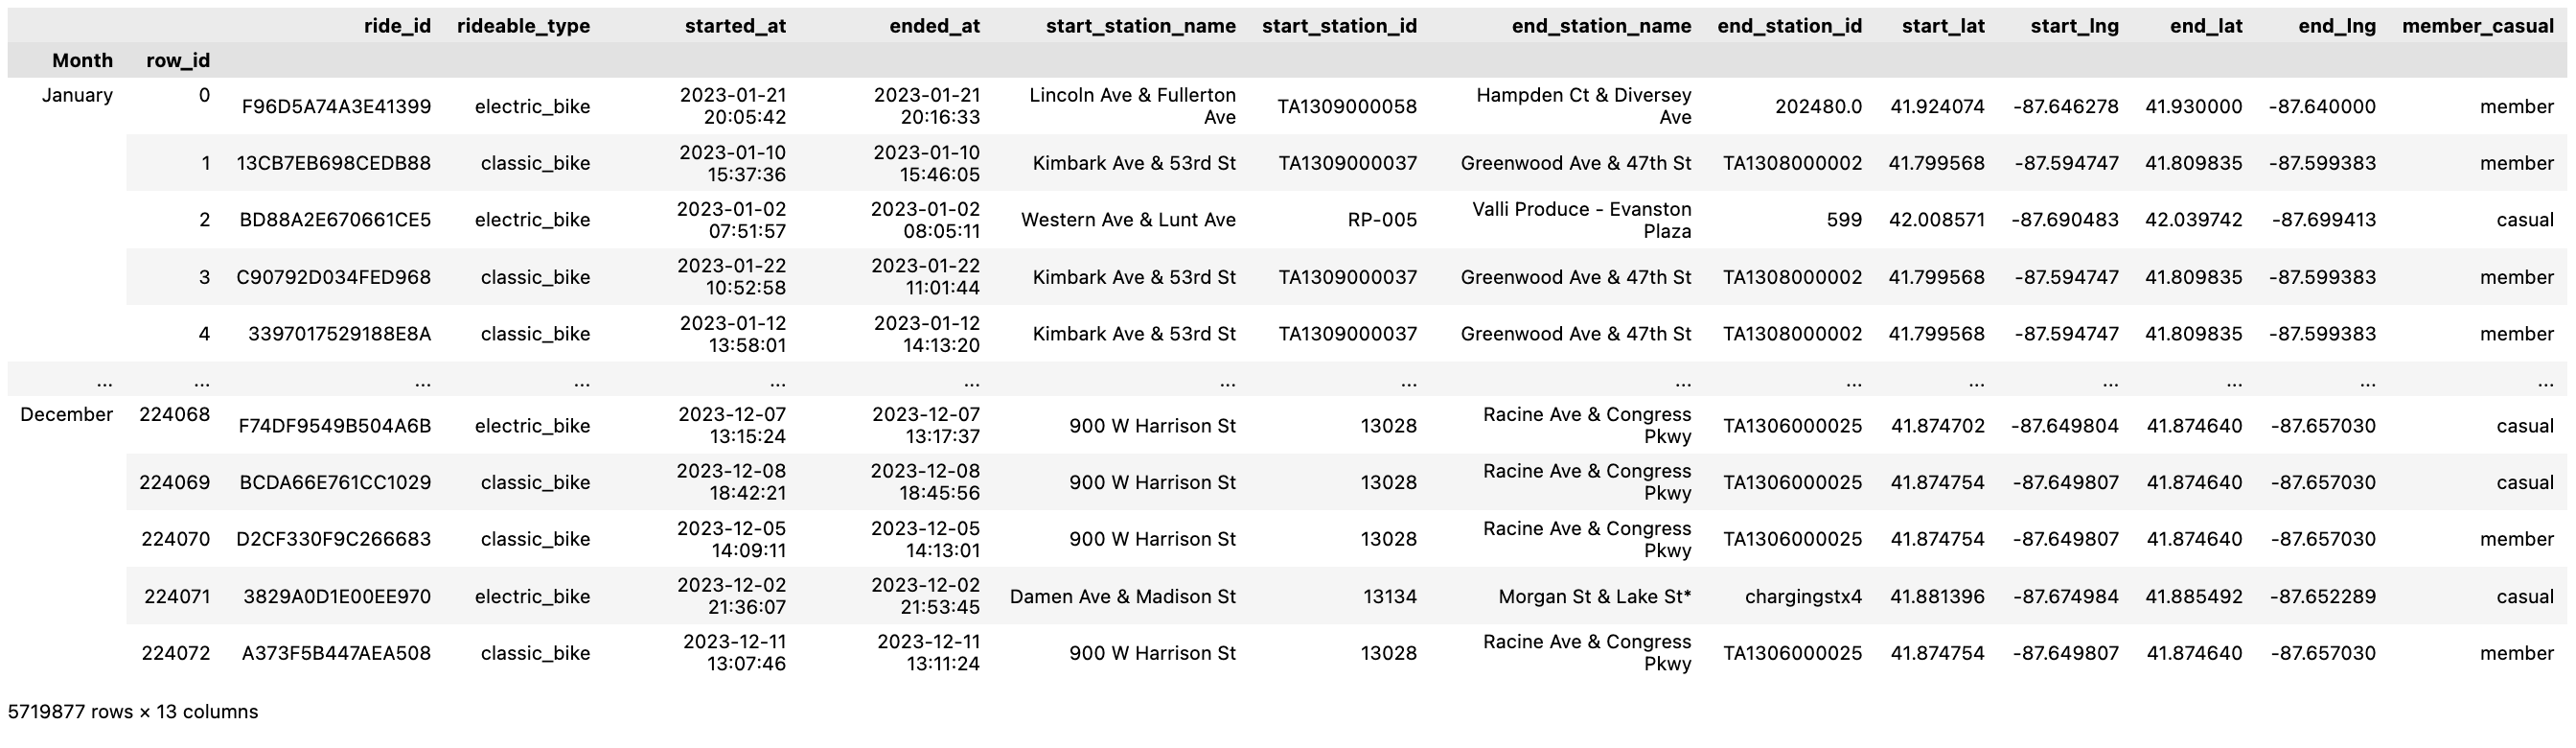
\includegraphics[scale=0.4]{original_data.png}
	\caption{First and last 5 entries of bike rides from the original data}
	\label{fig1}
	\end{figure}
	\pagebreak
	
	In Figure (\underline{\ref{fig1}}) the multi-index of the DF is shown in the first two columns (month, row\_id). Then looking at the entries themselves we can see that the data consists of 13 columns: 
	\begin{itemize}
	\item [1)] \textbf{ride\_id}: a unique identification string for each ride.
	\item [2)] \textbf{rideable\_type}: type of bike that was rented.
	\item [3-4)] \textbf{started(ended)\_at}: date and time for the start and end of the ride.
	\item [5-8)]  \textbf{start(end)\_station\_name(id)}: name and id of the start and end stations.
	\item [9-12)] \textbf{start(end)\_lat(lng)}: latitude and longitude of the start and end stations.
	\item [13)] \textbf{member\_casual}: whether the rider was an annual member or a casual rider.
	\end{itemize}

\section{Exploration}
Now that the files have been read and stored into a DF, the next step is to explore the dataset.
 
\subsection{Dataset size \& duplicates:}
First, we look at the size of the dataset by counting the number of bike rides in each month. The result is shown in Figure (\underline{\ref{fig3}}) along with its visualisation. On the left, we can see the exact number of bike rides for each month, the total number of bike rides in the dataset (year 2023), and the average per month. The dataset contains in total $\sim$5.7 Million entries, with an average of $\sim$480,000 rides per month. From the visualisation we can easily see that from November to April the number of rides is lower than the average, which is expected as these are cold months. This is confirmed by the peak in August. After retrieving this information for the original dataset, the duplicates were dropped, and the entries were counted again. The number of entries before and after turned out to be identical. Therefore the original dataset did not have any duplicates.\\ 
	
	\begin{figure}[h]
	\centering
	\begin{subfigure}{.3\textwidth}
	\hspace{-0.4 in}
		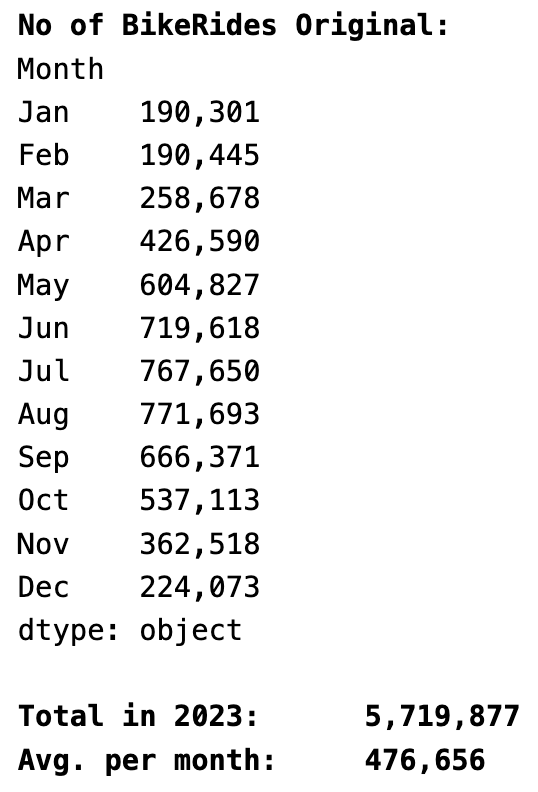
\includegraphics[scale=0.5]{no_of_rides_orig.png}
		%\caption{}
		%\label{fig3_1}
	\end{subfigure}
	\begin{subfigure}{.6\textwidth}
	\hspace{-0.8 in}
		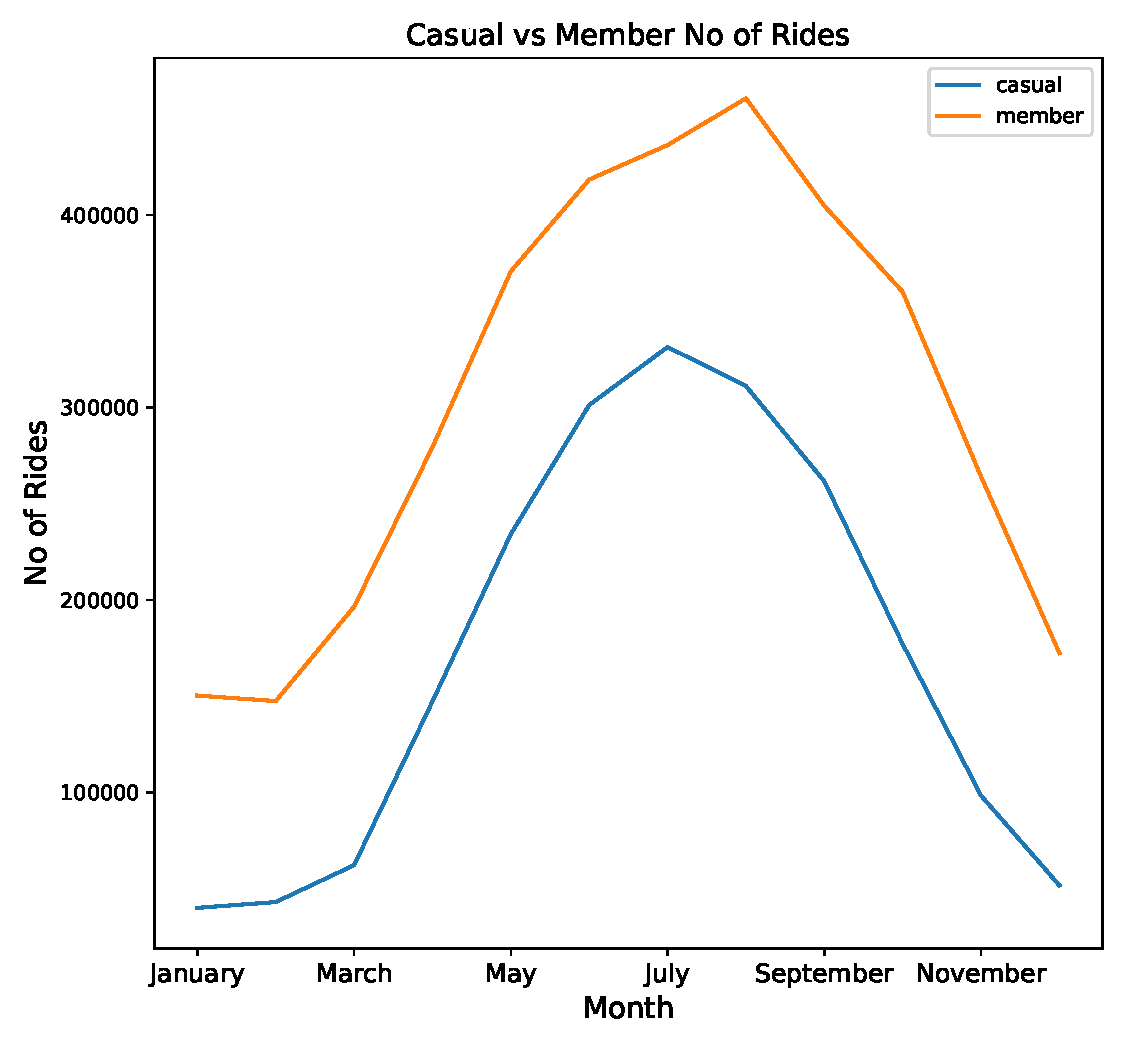
\includegraphics[scale=0.47]{no_of_rides.pdf}
		%\caption{}
		%\label{fig3_2}
	\end{subfigure}
	\caption{Dataset size}
	\label{fig3}
	\end{figure}

\subsection{Null values:}\label{sec1}
Next, we look at the percentage of null values for each column. First, the dataset is grouped by month, and then for each month, the percentage of null values in each column is calculated. The result is shown in Figure (\underline{\ref{fig4}}). As we can see the columns \textbf{start\_station\_name(id)}, \textbf{end\_station\_name(id)} in every month have 13-17\% null values. The columns \textbf{end\_lat(long)} have less than 1\% null values, and otherwise there are no null values. \\
	
	\begin{figure}[h]
	%\hspace{-0.5in}
	\centering
	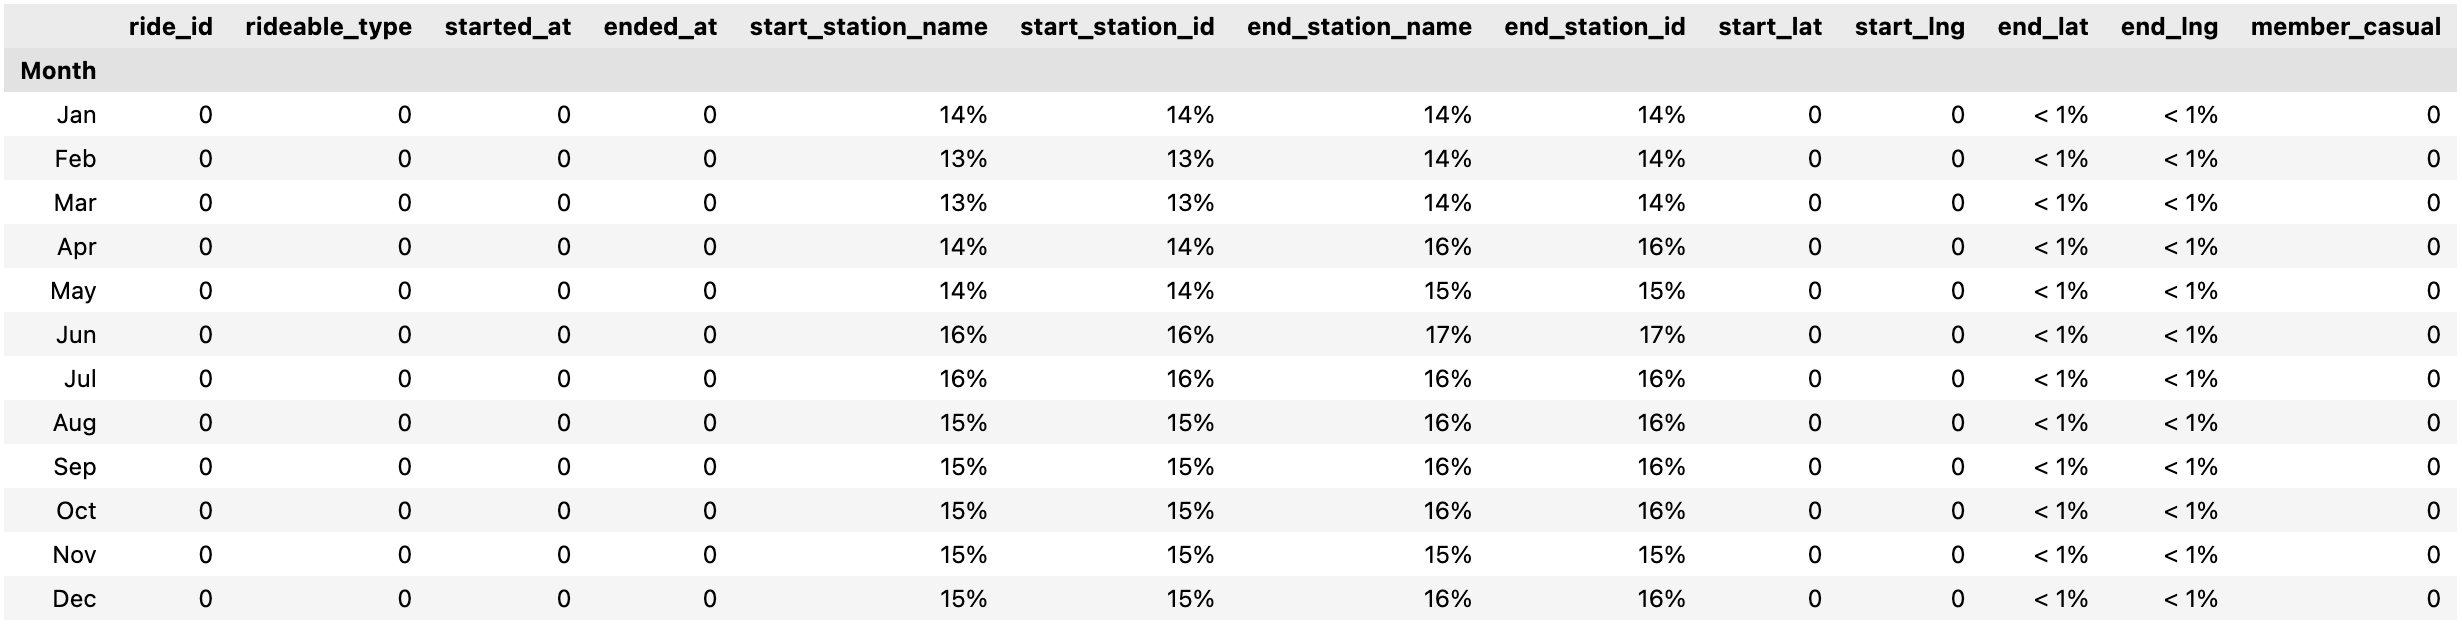
\includegraphics[scale=0.44]{null_percents.png}
	\caption{Percentage of null values per month}
	\label{fig4}
	\end{figure}
	
\subsection{Unique values:}\label{sec2}
Here we look at the unique (distinct) values for each column in the month of May. The unique values for several other months were inspected and there does not seem to be a significant difference, thus the choice of the month of May is random. The result is shown in Figure (\underline{\ref{fig2}}). 
	
	\begin{figure}[h]
	\centering
	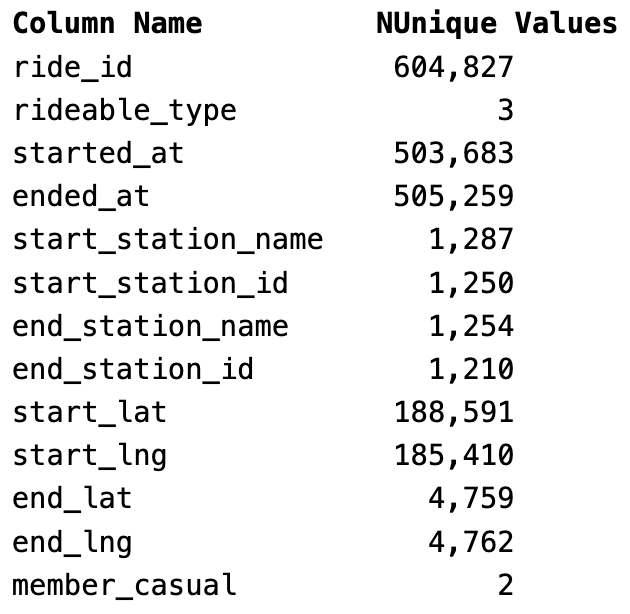
\includegraphics[scale = 0.6]{imgUni.png} 
	\caption{No. of unique values for every column in May}
	\label{fig2}
	\end{figure}
	
Next we investigate each unique value, knowing that the total number of rides in May is 604,827  (Fig. \underline{\ref{fig3}}):

	\begin{itemize}
	\item \textbf{ride\_id\_unique= 604,827}   \\
	As expected, \textbf{ride\_id} has as many unique values as the number of entries in the DF.
	\item \textbf{rideable\_type\_unique = 3}  \\
	These 3 values are the types of bikes that are offered by the company, which are: \\
	(electric/classic/docked).
	\item \textbf{started\_at\_unique = 503,683} , \textbf{ended\_at\_unique = 505,259} \\
	Seeing as how these columns are datetimes (yy-mm-dd hh:mm:ss), one may have expected them to have as many distinct values as the number of entries (604,827). However, the number of unique values in these columns is less than the number of entries by 16\%. Which means that 16\% of the bikes rides in May had the same \textbf{started\_at} as other rides. To explore this a bit further, one of these incidents has been retrieved and is shown in Figure (\underline{\ref{fig10}}). By looking at the entries, it is clear that they are indeed different rides (different start and end stations) but with the exact same start time. These unlikely incidents can be a result of having such a large dataset. For example, when looking at the entries in January, where there are a total of 190,301 rides we find that the percentage of rides with the same \textbf{started\_at} goes down to 6\%.  \\
	
	\begin{figure}[h]
	\hspace{0.3in}
	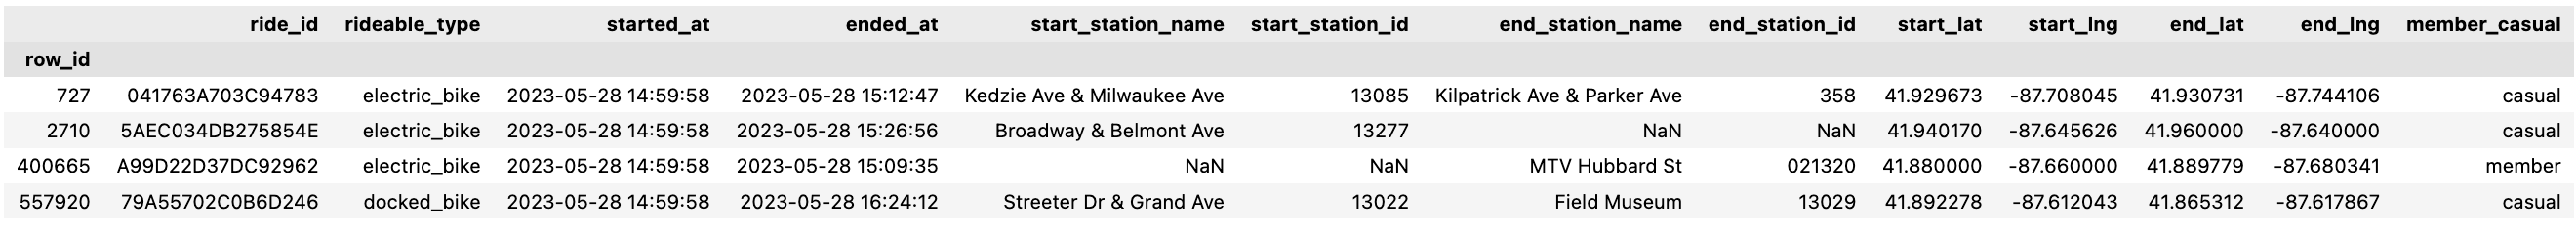
\includegraphics[scale=0.4]{imgDups1.png}
	\caption{Entries from May that have the same \textbf{started\_at} date and time}
	\label{fig10}
	\end{figure}
	
	\item \textbf{start\_station\_name(id)\_unique = 1287 and 1250}\\
	 \textbf{end\_station\_name(id)\_unique = 1254 and 1210} \\
	Since there is a limited number of stations, it is expected that these columns have a smaller number of unique values than the number of entries. However, one would have expected the number of unique station names and ids to be the same. Whereas the unique ids are less than the names by a small fraction. Which could either by accounted for by the null values (Fig. \underline{\ref{fig2}}) or could mean that there are stations that have the different names but the same id.
	
	\item \textbf{start\_lat(long)\_unique = 188,591 and 185,419} \\
	\textbf{end\_lat(long)\_unique = 4759 and 4762} \\
	The start latitude and longitude numbers seem to be as expected, which is less than the total number of entries, but more than the number of stations (this is based on the assumption that the exact location where a bike is parked can vary within the station especially that the values are given to the $6^{th}$ decimal place). However, there is a large difference between the number of values in the \textbf{start\_lat(long)} ($\sim$188,000) and the numbers in the \textbf{end\_lat(long)} ($\sim$4800). This difference cannot be accounted for by the null values in the end columns, since these were less than 1\%. If these values are true, that would mean that users rode there bikes from many start locations, but mostly ended up in a much smaller set of locations. Which cannot be the case since that would have been reflected in a similar difference between the number of \textbf{start\_station\_name} and \textbf{end\_station\_name} stations. This discrepancy occurs in all 12 months. 
	\item \textbf{member\_casual\_unique} = 2 \\
	These 2 values are the types of riders, which are: (casual/member).
	\end{itemize}

	
\section{Cleaning}
After exploring the dataset, we can see that the extractable information can be divided into information about the:
	\begin{enumerate} 
	\item rider (casual/member).
	\item bike (electric/classic/docked).
	\item ride (start-end: time, date, location).
	\end{enumerate}

\subsection{Drop columns:}
The only columns that had null values and discrepancies were the ones related to the ride location. Assuming that the amount paid by the rider is based on how long in time the bike was rented, then the information related to the ride length can be extracted from the columns \textbf{started\_at} and \textbf{ended\_at} and the columns related to the ride location can then be dropped. The column \textbf{ride\_id} will also be dropped as it does not provide any valuable information for the current analysis and is rendered redundant by the index \textbf{row\_id}. \\

\subsection{Data formatting:}
After dropping the columns related to the ride location and ride id, we are left with the columns:
\begin{itemize}
	\item \textbf{rideable\_type}
	\item \textbf{member\_casual}
	\item \textbf{started\_at}
	\item \textbf{ended\_at}
\end{itemize}
We have already looked at the columns \textbf{rideable\_type} and \textbf{member\_casual}, and ensured that they have no null values (Sec. \underline{\ref{sec1}}) and only the expected values (Sec. \underline{\ref{sec2}}). As for the columns \textbf{started\_at} and \textbf{ended\_at}, these do not have null values, but still need to be checked to ensure that the \textbf{ended\_at} time always comes after \textbf{started\_at} time. In order to do that, these columns are first converted from strings of characters to a numerical date-time format. Next, the rides where the \textbf{ended\_at} time is before the \textbf{started\_at} time are filtered and shown in Figure (\underline{\ref{fig8}}). In the entire dataset of $\sim$5.7 Million entries, there is a total of 272 entries that have this issue. Since, the dataset is large, the entries are simply dropped. \\

	\begin{figure}[h]
	\centering
	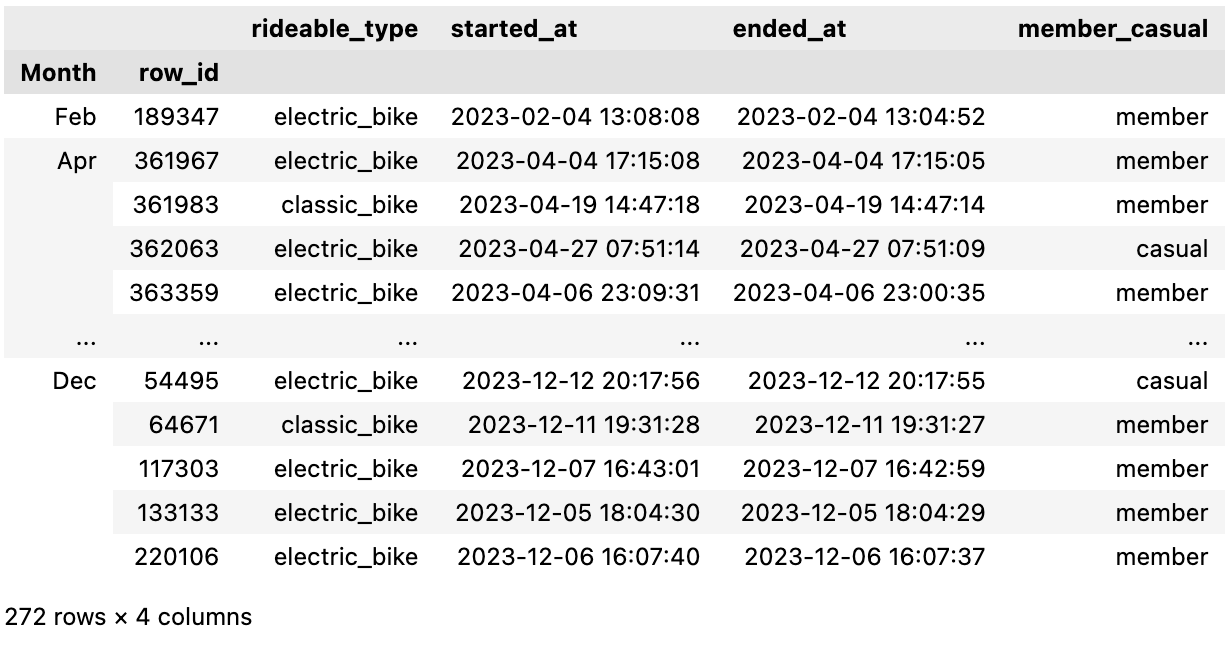
\includegraphics[scale=0.5]{same_started_at.png}
	\caption{Entries where the \textbf{ended\_at} time is before the \textbf{started\_at} time}
	\label{fig8}
	\end{figure}
	
	
\section{Preparation}
In order to prepare the data for analysis, two new columns are added. First is \textbf{ride\_length}: the difference between the columns \textbf{ended\_at} and \textbf{started\_at} times. Second is \textbf{day\_of\_week}: extracted from the date in \textbf{started\_at}. The columns \textbf{started\_at} and \textbf{ended\_at} are then dropped, since the new columns make them redundant.
	

\section{Analysis}
Finally, the data can be analysed in order to determine how casual riders and members use the bikes differently.

\subsection{Number of rides:}
We have already seen the number of rides per month in Figure (\underline{\ref{fig3}}). Now we will look at the same information, however this time per rider type; i.e member/casual. In order to do this, a pivot table is produced where the index is the month, and the values are the number of rides per rider type. This table is shown in Figure (\underline{\ref{fig17}}) along with its visualisation. Below the pivot table, we can see the total number of rides in the year 2023 per rider type. Here we see that of 5.7 Million rides, 36\% were by casual riders, and 64\% were made by members. In the plot we see the number of rides as stacked bars; i.e. the number of rides for annual members stacked ontop of the number of rides for casual riders.  From the plot we observe that, rides by members and casual riders follow the same pattern of peaking during the summer months, and dropping during the winter months. However, we see that the percentage of casual riders to members fluctuates throughout the year. In January there were 21\% rides by casual riders, and 79\% by members, whereas in August there were 40\% rides by casual riders, and 60\% by members. \\
\newline

	\begin{figure}[h]
	\begin{subfigure}{.3\textwidth}
	%\hspace{-0.4 in}
		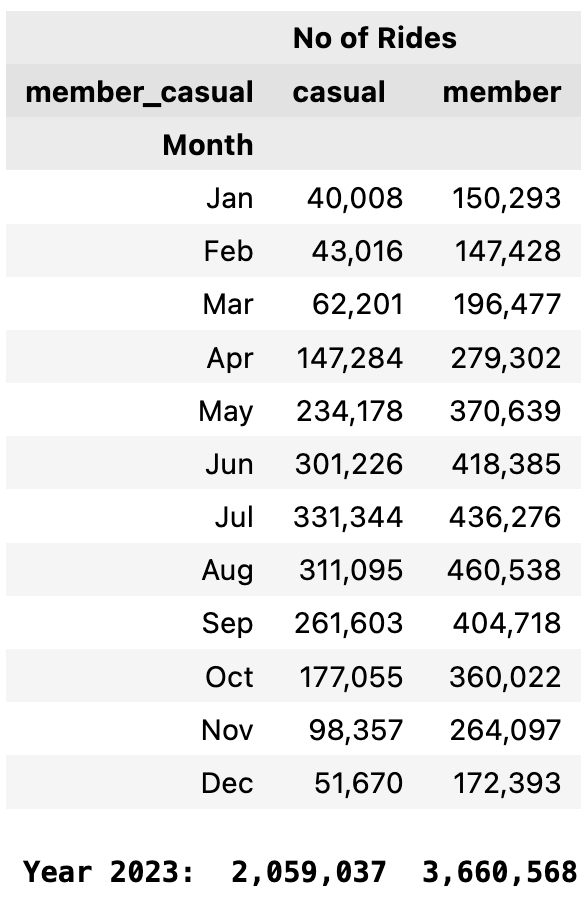
\includegraphics[scale=0.5]{no_of_rides_per_rider.png} 
	\end{subfigure}
	\begin{subfigure}{.6\textwidth}
	\hspace{-0.35in}
		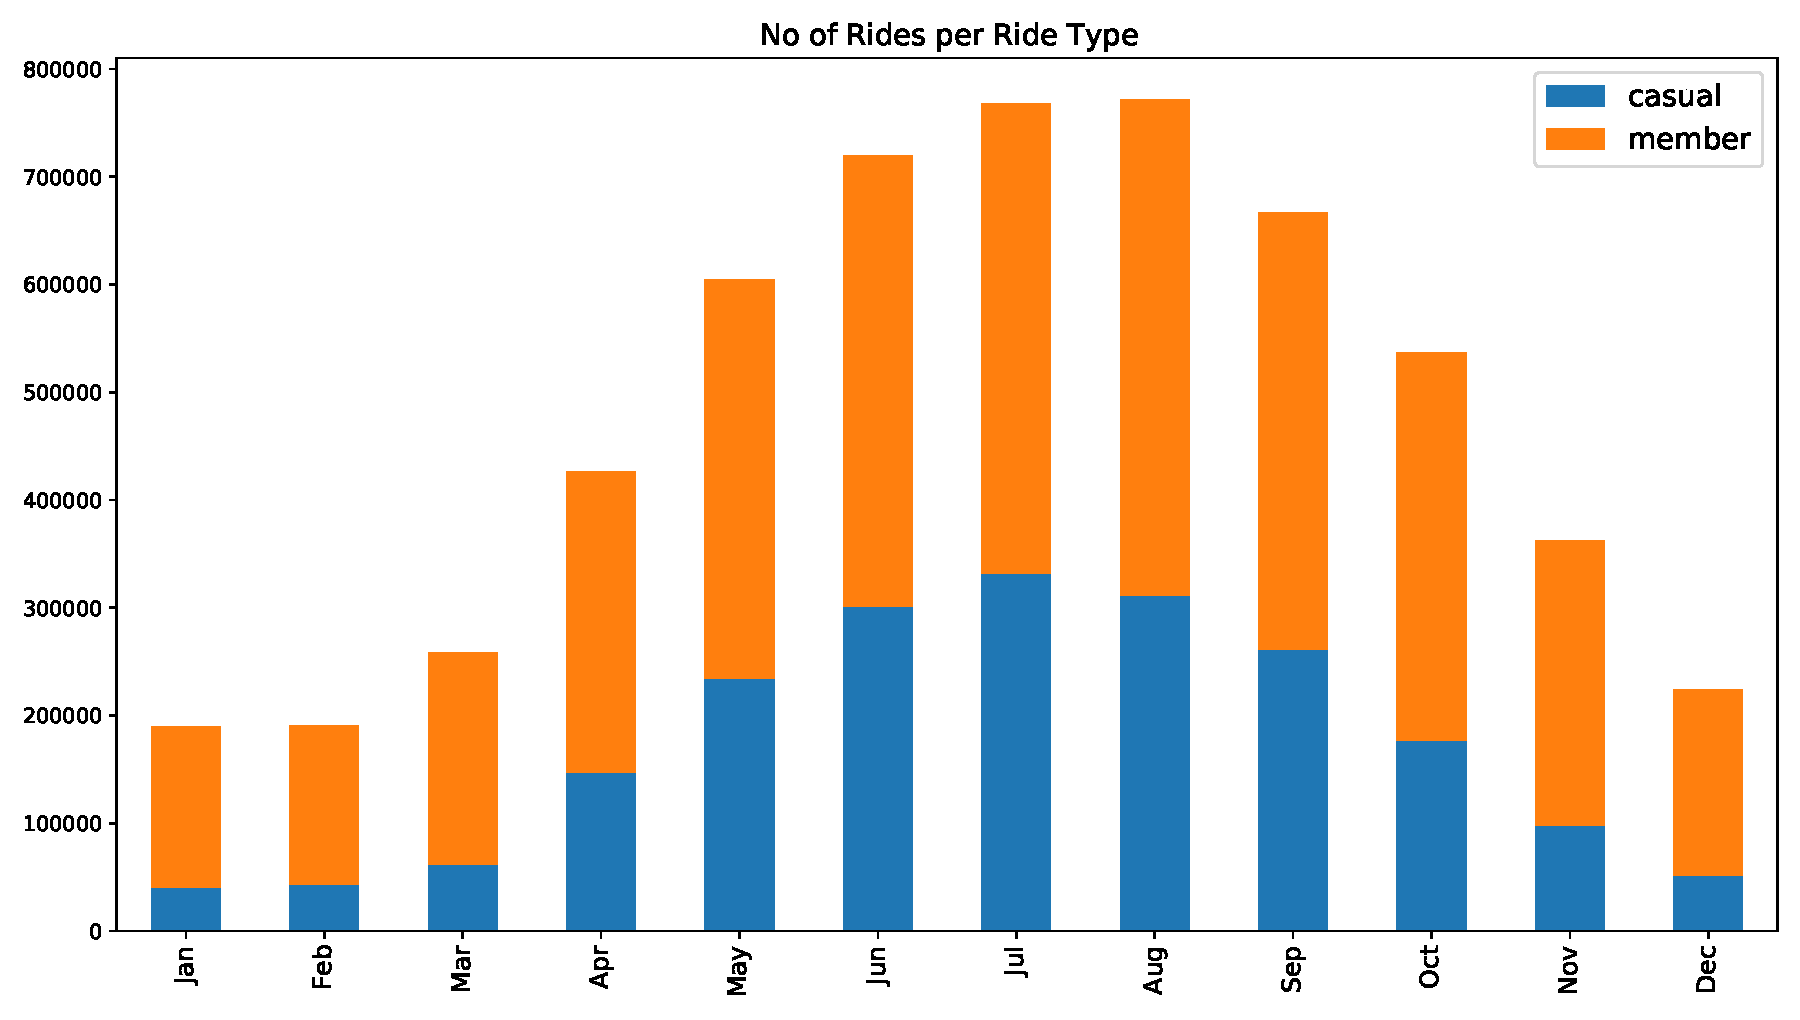
\includegraphics[scale=0.46]{no_of_rides_per_rider_type.pdf}
	\end{subfigure}
	\caption{No. of rides per rider type. Left: Pivot table. Right: Stacked bar chart}
	\label{fig17}
	\end{figure}
	
\subsection{Ride length mean and maximum:}\label{sec3}
\subsubsection*{Dataset Groupedby Month:}
In order to look at the mean and maximum ride length per rider type, a pivot table is used and is shown along with the corresponding visualisations in Figure (\underline{\ref{fig11}}). It should be noted that although it would have been more consistent to continue using bar charts, the choice was made here to use line plots as they visualised the information more clearly and appeared less crowded. The bar charts have been produced nevertheless and can be found in the Appendix (\underline{\ref{app1}}). From the line plot of the mean values in Figure (\underline{\ref{fig11_2_1}}) we observe that casual riders have longer rides, than members across the entire year. Also, the mean ride length for casual riders varies across the year from approximately 20 minutes in the colder months to a peak of 35 minutes in August. As for members, their mean ride length changes only from 10 minutes in the colder months to 13 minutes in peak months. \\

When looking at the maximum ride length plot in Figure (\underline{\ref{fig11_2_2}}) we see a similar pattern: casual riders have longer rides, and their maximum ride lengths changes significantly over the year from 1 day in the cold months to 68 days in August. As opposed to, members whom have a maximum ride length of 1 day all throughout the year. 
	\begin{figure}[h]
	\centering
		\begin{subfigure}[b]{0.55\textwidth}
   			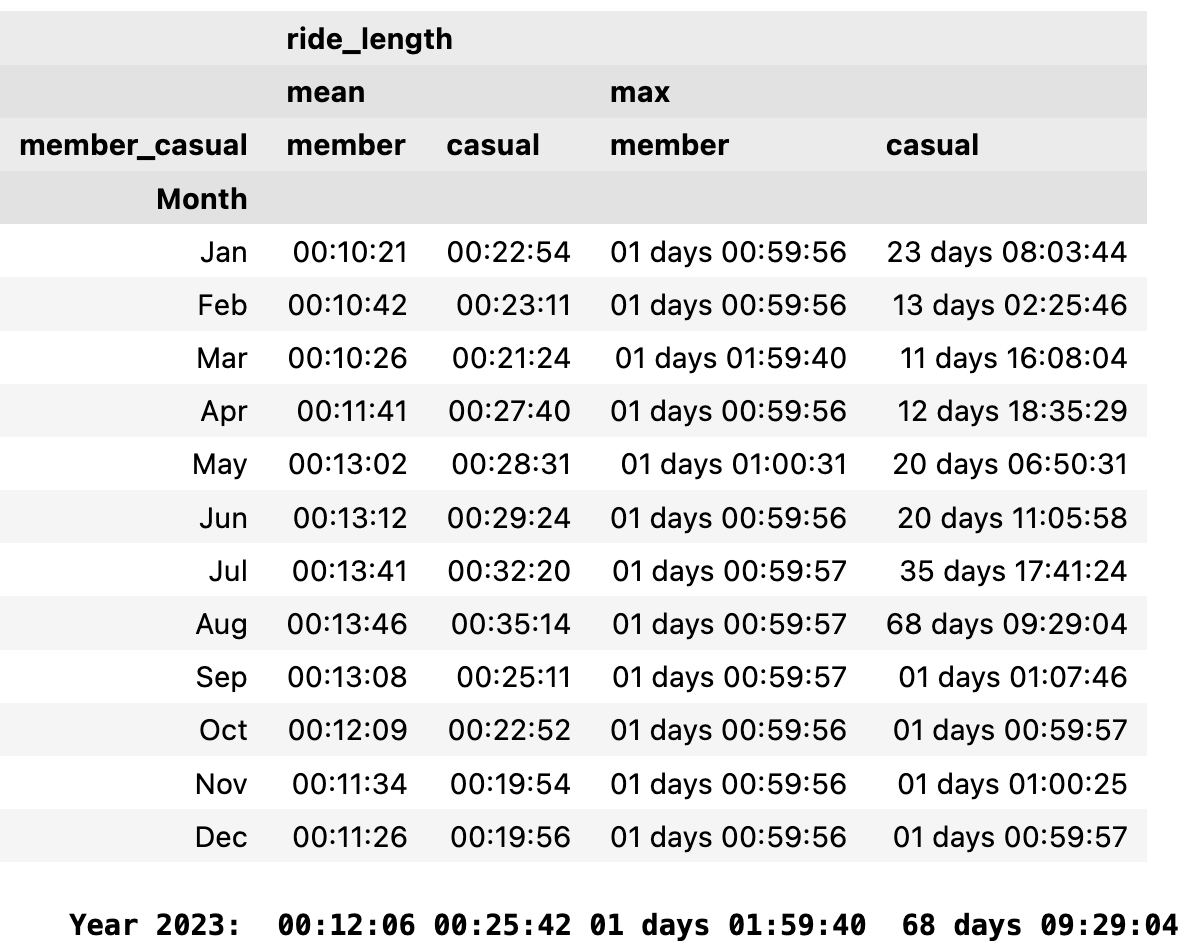
\includegraphics[scale=0.5]{mean_max.png} 
		\end{subfigure}

		\begin{subfigure}[b]{0.55\textwidth}
			\hspace{-1.5in}
   			\begin{subfigure}{.45\textwidth}
				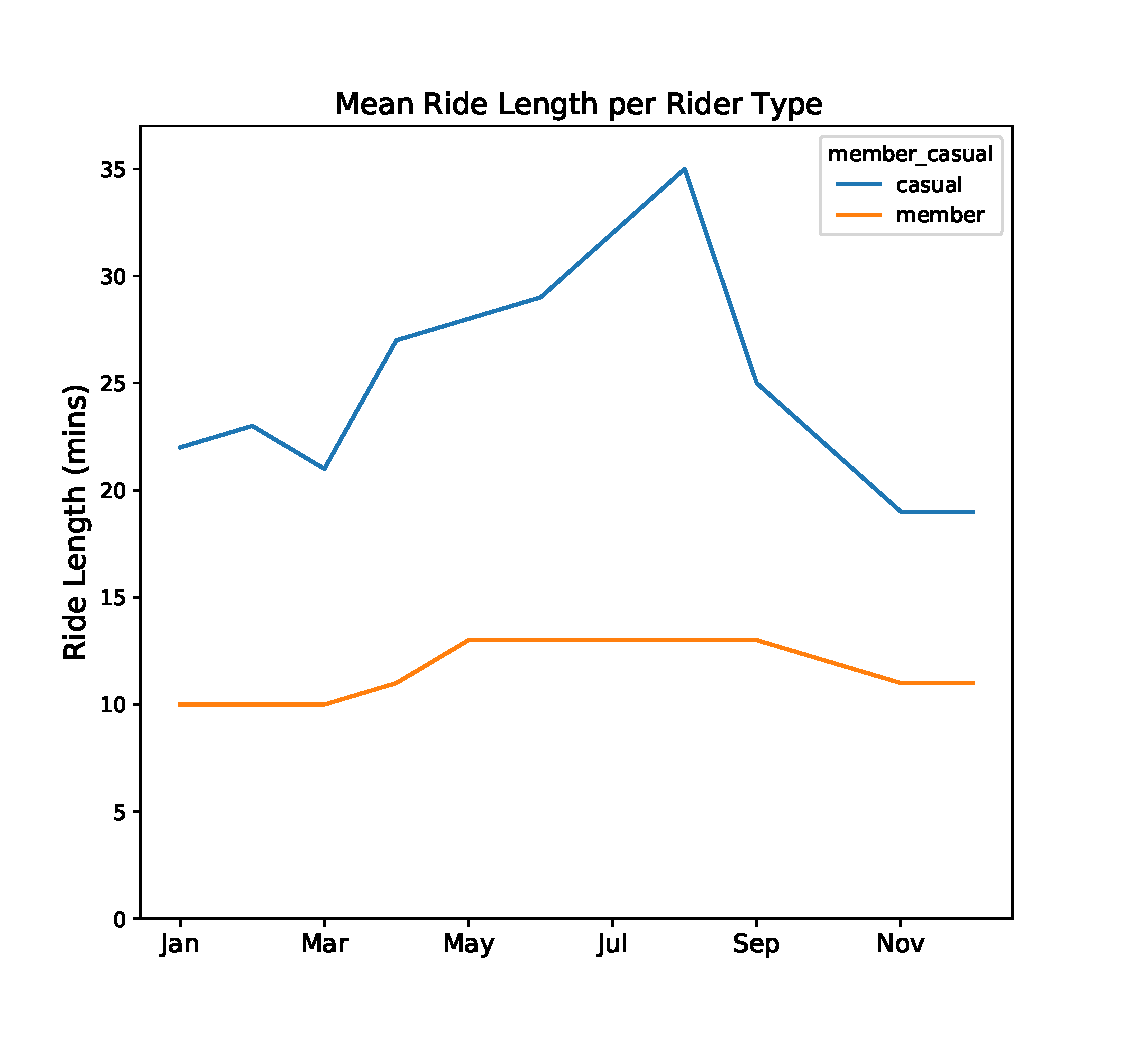
\includegraphics[scale=0.5]{mean_ridelength_line.pdf} 
				\caption{}
				\label{fig11_2_1}
			\end{subfigure}
			\hspace{1.5in}
			\begin{subfigure}{.4\textwidth}
				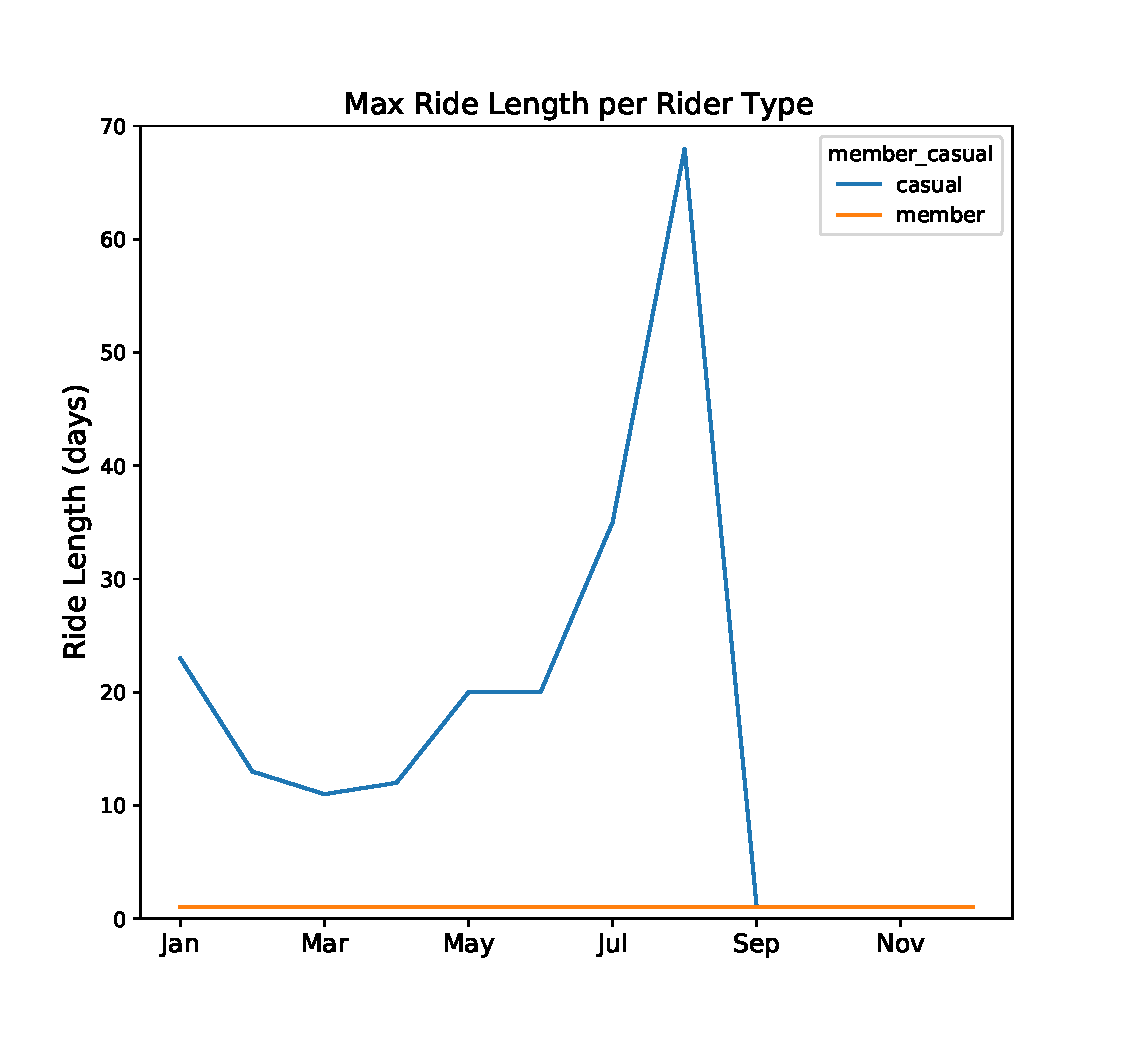
\includegraphics[scale=0.5]{max_ridelength_line.pdf} 
				\caption{}
				\label{fig11_2_2}
			\end{subfigure}
		\end{subfigure}
		\caption{Mean and max ride length divided by rider type. Top: Pivot table. Bottom: Line plots}
		\label{fig11}
	\end{figure}

\pagebreak

\subsubsection*{Entire Dataset Distribution:}
When looking at the values in the maximum ride length plot in Figure (\underline{\ref{fig11_2_2}}), we see that casual riders have significantly longer rides than members. In order to see, how much of the entire population do such large values actually represent, the entire dataset of ride lengths is visualised using a box plot as shown in Figure (\underline{\ref{fig13}}).  

	\begin{figure}[h]
	\centering
	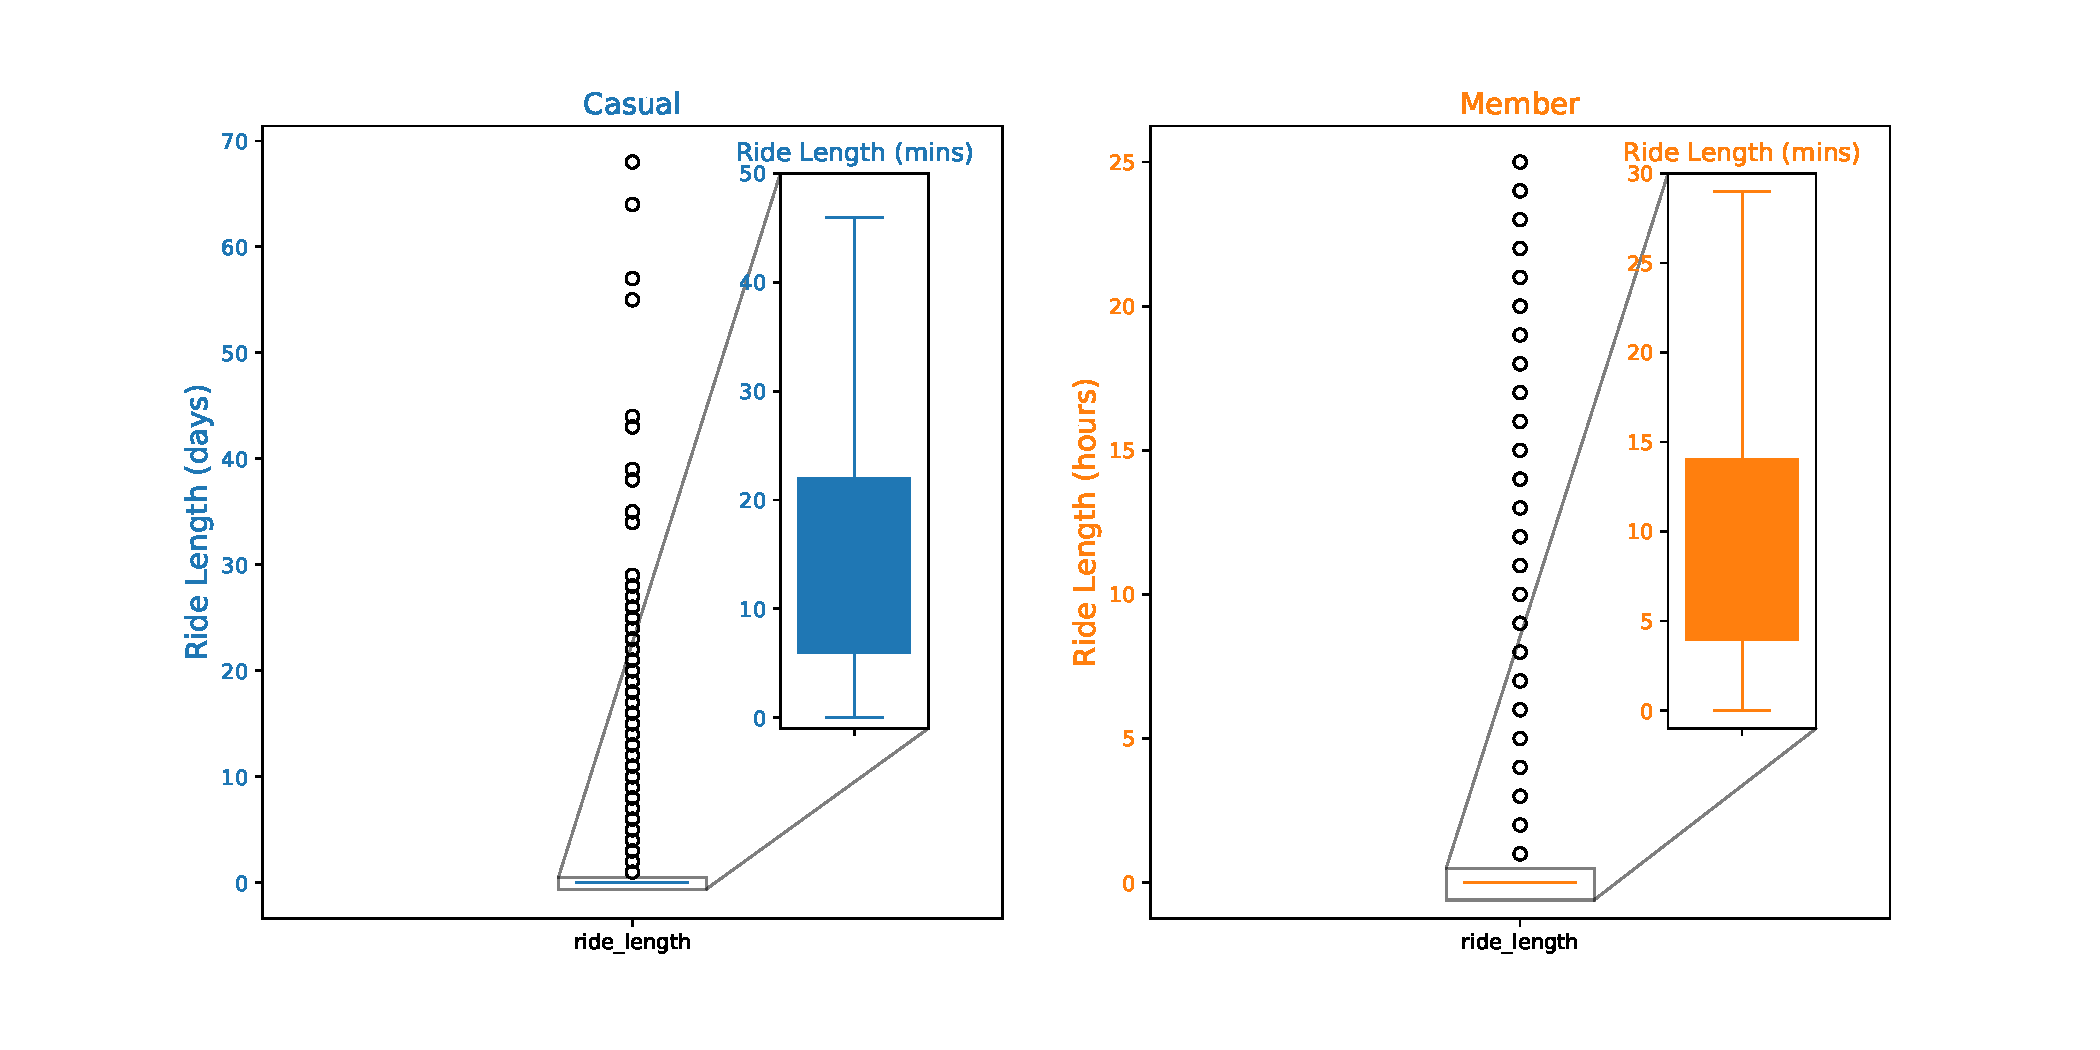
\includegraphics[scale=0.5]{ridelength_boxplot.pdf} 
	\caption{Distribution of ride length values visualised using box plots}
	\label{fig13}
	\end{figure}
	
A box plot typically divides the values in a distribution into 4 quartiles (0-25\%, 25-50\%, 50-75\%, 75-100\%), and displays them as follows: 
	\begin{itemize}
	\item the middle 2 quartiles (25-75\%) are shown inside a box.
	\item the lower and upper quartiles (0-25\%,75-100\%) are shown by whiskers.
	\item outliers are shown using circles. 
	\end{itemize}
From Figure (\underline{\ref{fig13}}) left, we can see that for casual riders, the outlier points are the ones that occupy the range [1 - 70] days, whereas the distribution itself can only be seen in the [0 - 50] minute range. As for the members, the distribution of ride lengths is in the [0 - 30] minute range, and its outliers are in the [1- 25] hour range. This tells us that, significantly longer rides as those that appear in the maximum ride plot Figure (\underline{\ref{fig11_2_2}}), are outliers that occur quite rarely and should not be used to draw conclusions about the general behaviour of casual riders. Therefore, in order to see the comparison between the ride lengths for casual riders and members more clearly, the box plots are populated once more after dropping the outliers in Figure (\underline{\ref{fig15}}).  \\

	\begin{figure}[h]
	\centering
	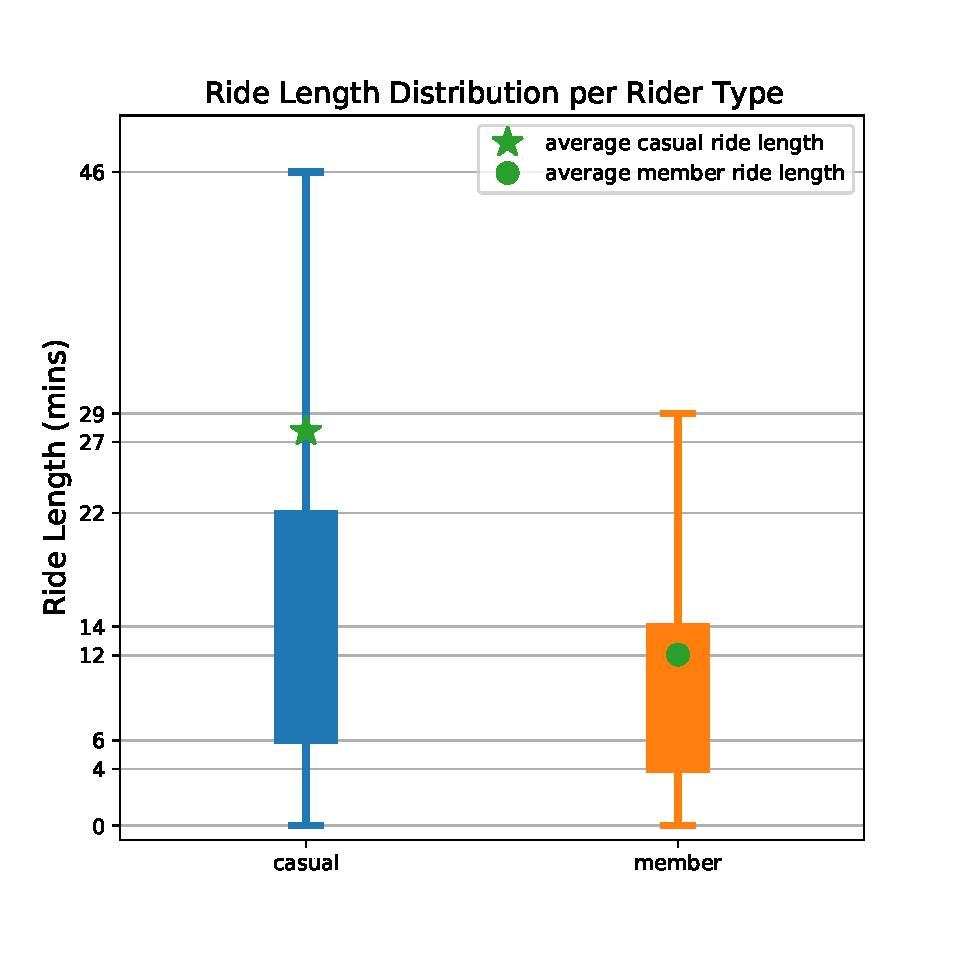
\includegraphics[scale=0.6]{ridelength_boxplot_wo_outliers.pdf} 
	\caption{Comparison between the ride lengths of casual riders and members without outliers}
	\label{fig15}
	\end{figure}

Figure (\underline{\ref{fig15}}) gives a more detailed comparison of the distribution of casual riders and members. The main distribution of ride lengths for casual riders varies between [0 - 46] minutes, as opposed to [0 - 29] minutes for members. If we look at the middle 50\% of casual rider values, these are between [6 - 22] minutes, whereas members are between [4 - 14] minutes. The mean values calculated from the entire distribution are also marked on the plot using green markers. For casual riders the mean is 27.7 minutes (slightly higher than the mean calculated first by month and then for the year 2023 in Fig. (\underline{\ref{fig11}}) = 25.7 ), and for members it is 12 minutes.  

\pagebreak
\subsubsection*{Dataset Groupedby Day of Week:}
So far we have compared the mean ride length of rider types either by first grouping the data using the month (Fig. \underline{\ref{fig11_2_1}}) or by looking at the entire distribution (Fig. \underline{\ref{fig15}}). In order to get a different perspective, we will now look at the mean value of the ride length after the data has been grouped by the day of the week. The resulting pivot table as well as its visualisation are shown in Figure (\underline{\ref{fig14}}). Here we see the same higher average for the casual riders when compared to members. Another observation is that casual riders exhibit a peak during the weekend and a drop during the middle of the week. 
	
	\begin{figure}[h]
	\hspace{0.8in}
	\begin{subfigure}{.2\textwidth}
		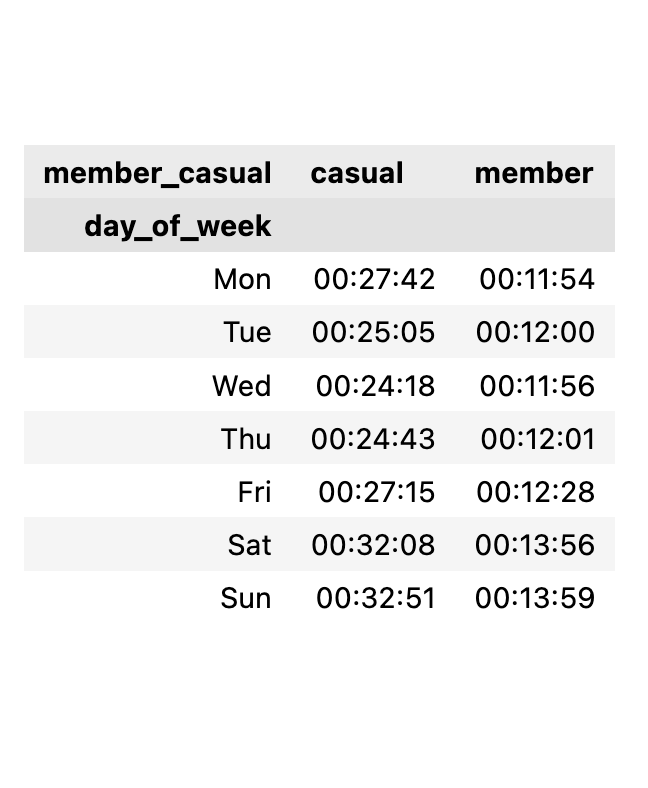
\includegraphics[scale=0.53]{dayofweek_t.png} 
	\end{subfigure}
	\begin{subfigure}{.55\textwidth}
	\hspace{1.2in}
		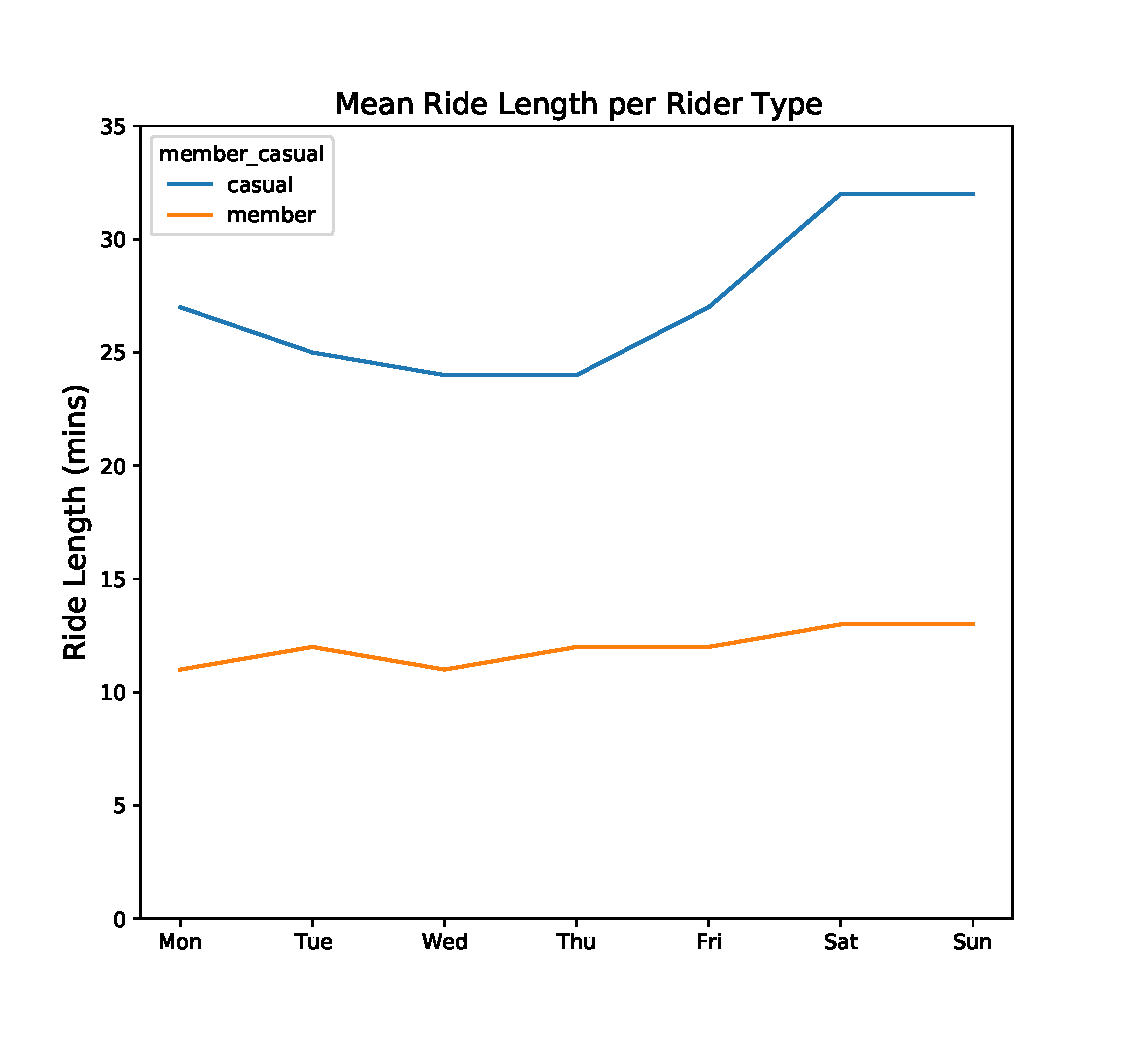
\includegraphics[scale=0.43]{mean_ridelength_line_dayofweek.pdf}
	\end{subfigure}
	\caption{Mean ride length per rider type grouped by day of the week}
	\label{fig14}
	\end{figure}
	\pagebreak

\subsection{Type of bike:}
Finally, here we look at the types of bikes rented by casual riders and members. This is done by looking at the number of entries in each category in the column \textbf{rideable\_type}. The result is visualised in Figure (\underline{\ref{fig16}}). From the bar chart we can see that for classic and electric bikes, there are more member rides than casual rides. Which is to be expected, since the overall number of member rides is larger than the casual riders (Fig. \ref{fig17}). However, the interesting finding is that when it comes to docked bikes, only casual riders have used those in 2023.
	
	\begin{figure}[h]
	\centering
	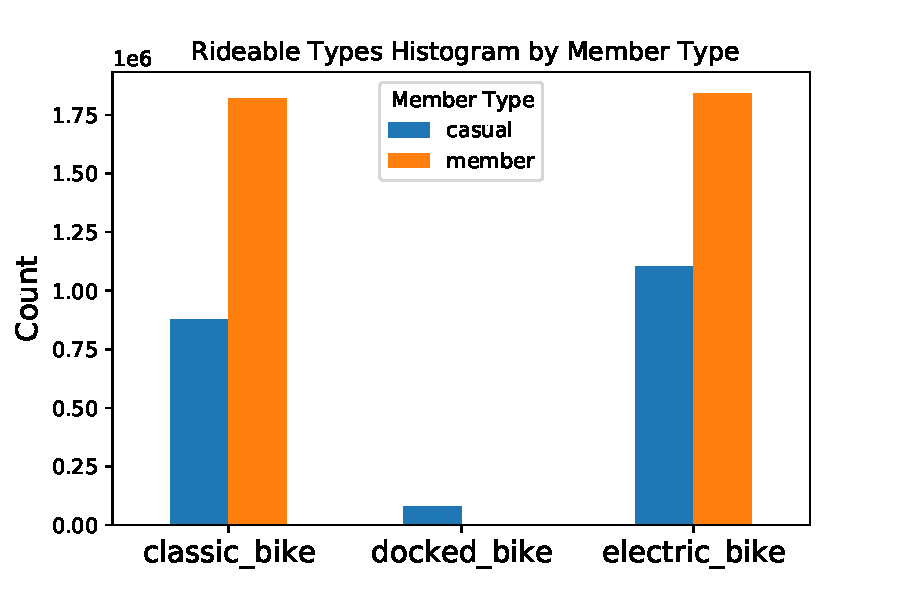
\includegraphics[scale=0.6]{rideable_types.pdf} 
	\caption{No of Rides for each type of bike}
	\label{fig16}
	\end{figure}
	

%\pagebreak

\section{Conclusion}

In this report, the analysis of a bike-sharing case-study was presented. First, the dataset was explored by looking at   what the original data consisted of, what were the unique values in each column, as well as the percentage of null values. For the year 2023, on average, there were $\sim$480,000 rides per month. During the cold months December-February the rides dropped to $\sim$200,00, and in the summer months they went up to $\sim$770,000 rides. No duplicates were found in the dataset, but the columns \textbf{start(end)\_station\_name(id)} had 13-17\% null values, and the columns \textbf{end\_lat(long)} had less than 1\% null values. When looking at the number of unique values for each column, some discrepancies were found, for example there were $\sim$188,000 start locations (latitude and longitude) whereas there only $\sim$4800 end locations. Next, the data was cleaned by dropping the columns that had inconsistencies, null values or were irrelevant to the analysis. The data was also formatted by converting the start and end times into date-time numerical values and the entries where the end time was before the start were dropped. In order to prepare the data for analysis, the columns \textbf{ride\_length} and \textbf{day\_of\_week} were added. \\

The data was then analysed by first looking at the number of rides performed by members versus casual riders. The entire dataset for the year 2023 consists of 5.7 Million rides, 64\% of which were made by annual members, and 36\% were by casual riders. The dataset was then grouped by month, and the average and maximum ride length were calculated per rider type. For members the mean ride length in 2023 was $\sim$12 minutes, whereas for casual riders it was $\sim$25 minutes. When looking at the maximum ride length it was shown that members never rented the bike for more than one day, whereas casual riders had a maximum ride length ranging from 1 - 68 days. However, by plotting the entire distribution of ride length values using box plots, it was shown that such longer rides were outliers that occurred quite rarely. The box plots showed that the main distribution of ride lengths after ignoring the outliers can be summarised by the values shown in Table (\underline{\ref{table1}}): 

\begin{table}[h]
\begin{center}
\begin{tabular}{ | c | c | c| c | c |  } 
\hline
   	& 0 - 25\% 	& 25 - 70\% 	& 75 - 100\% &  mean (mins)  \\ 
  \hline
casual 	& 0 - 6 		&  6 - 22 		& 22 - 46 & 27 \\
\hline
member 	& 0 - 4 		& 4 - 14		& 14 - 29 & 12 \\
\hline
\end{tabular}
\caption{Distribution of ride lengths for casual riders and members without outliers}
\label{table1}
\end{center} 
\end{table}


By looking at the results shown in Table (\underline{\ref{table1}}) we can confidently conclude that casual riders have longer ride lengths, whether we compare the mean across the whole dataset, or if we compare each quartile of the distribution. Therefore, this analysis supports the recommendation to target converting casual riders into members. Lastly, it was found that in the year 2023, docked bikes were used only by casual riders.

\pagebreak
\section{Appendix}

\subsection{Ride length mean and maximum:}\label{app1}
The mean and maximum ride lengths per rider type are shown here using bar charts. 

	\begin{figure}[h]
   		\begin{subfigure}{.45\textwidth}
		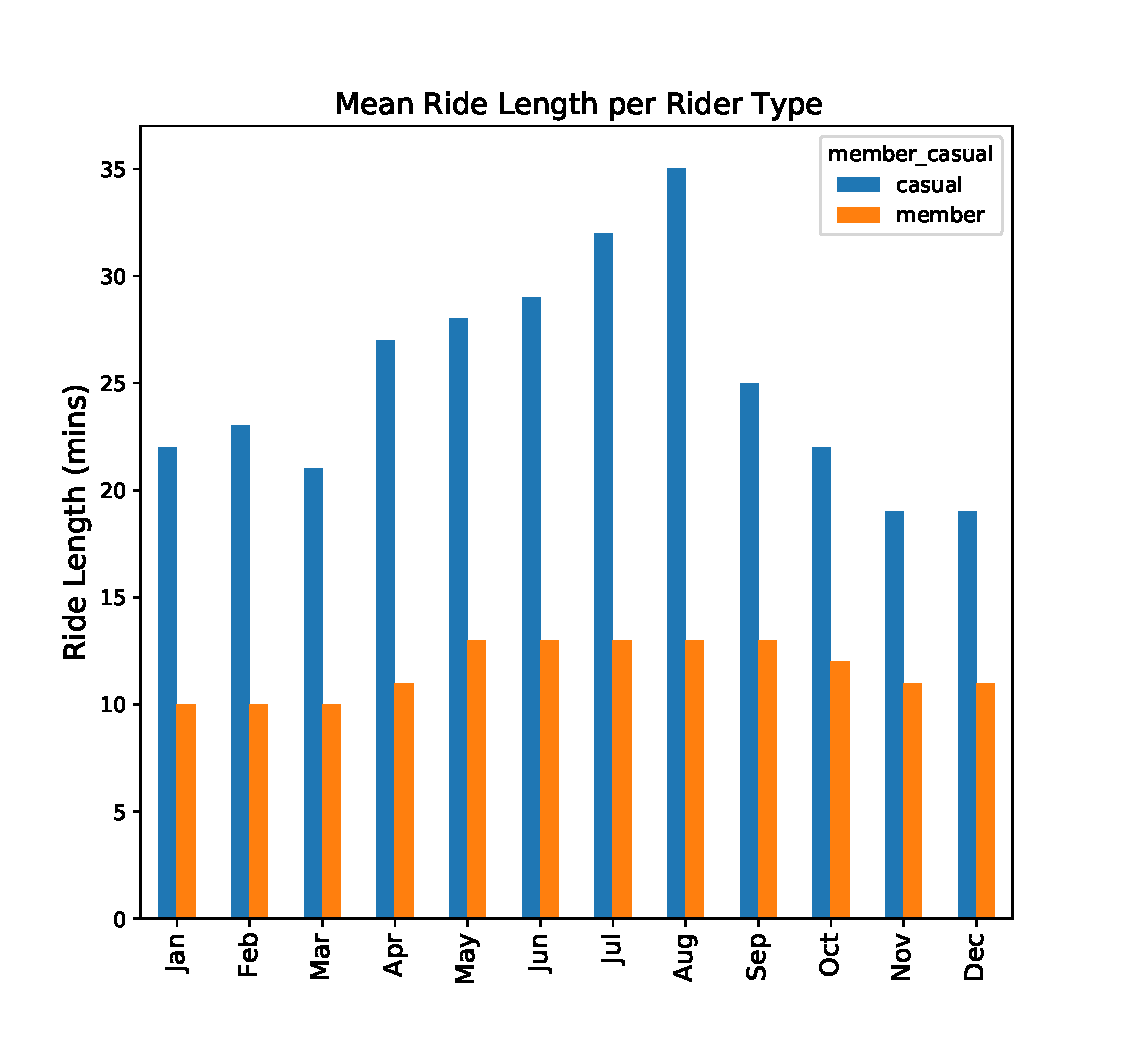
\includegraphics[scale=0.5]{mean_ridelength_bar.pdf} 
		\end{subfigure}
		\hspace{0.5in}
		\begin{subfigure}{.4\textwidth}
		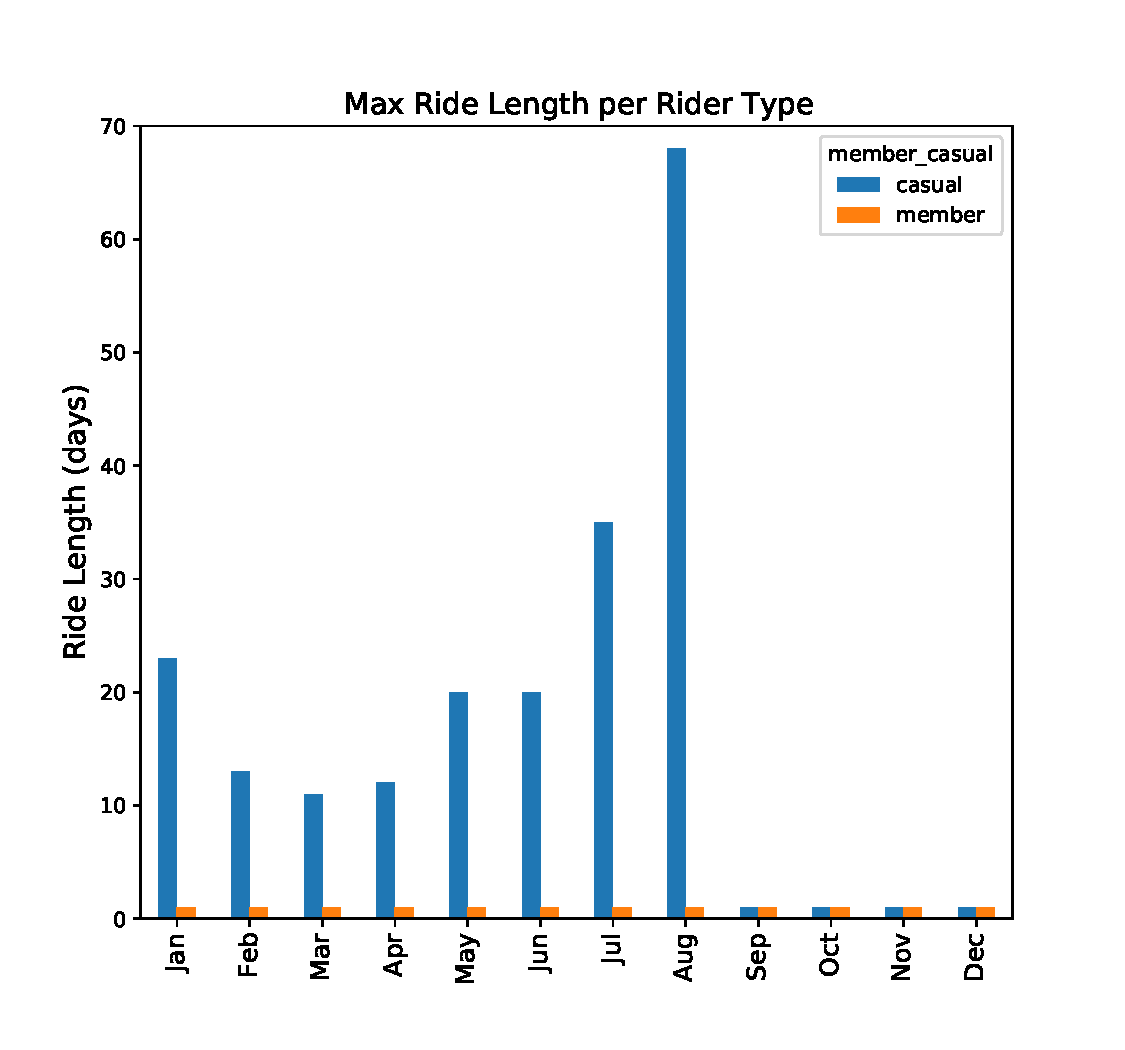
\includegraphics[scale=0.5]{max_ridelength_bar.pdf} 
		\end{subfigure}
		\caption{Mean and maximum ride length bar charts}
	\end{figure}


\end{document}